\subsection*{Anhang}\label{anhang}
\setcounter{page}{1}
\paragraph{Environment - Agenteninput}\label{anh_env_bilder_chaser} \hfill \break
Folgend werden die Environment-Konfigurationen gezeigt, die über den Verlauf der Experimente verwendet wurden.
\begin{figure}[htb!]
   \captionsetup{width=0.30\linewidth} 

    \begin{minipage}{0.3\linewidth}
        \centering
        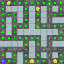
\includegraphics[scale=1.2]{abb/_envpics/example_green}
        \caption*{Default Spiel}
        \label{fig:pic_chaser_defautl}
    \end{minipage}
    %\hfill
    \begin{minipage}{0.3\linewidth}
        \centering
        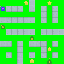
\includegraphics[scale=1.2]{abb/_envpics/example_greenBG}
        \caption*{Hintergrund grün}
        \label{fig:pic_chaser_greenBG}
    \end{minipage}
    \begin{minipage}{0.3\linewidth}
        \centering
        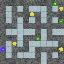
\includegraphics[scale=1.2]{abb/_envpics/example_noVisOrb}
        \caption*{Keine vis. Orbinformation}
        \label{fig:pic_chaser_noVisOrb}
    \end{minipage}
    %\caption{Chaser Environment - links unskaliert, rechts skaliert}
\end{figure}

\begin{figure}[htb!]

   \captionsetup{width=0.30\linewidth} 
    \begin{minipage}{0.3\linewidth}
        \centering
        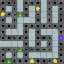
\includegraphics[scale=1.2]{abb/_envpics/example_black}
        \caption*{Schwarze Orbs}
        \label{fig:pic_chaser_blackOrb}
    \end{minipage}
    %\hfill
    \begin{minipage}{0.3\linewidth}
        \centering
        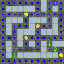
\includegraphics[scale=1.2]{abb/_envpics/example_blue}
        \caption*{Blaue Orbs}
        \label{fig:pic_chaser_blueOrb}
    \end{minipage}
    \begin{minipage}{0.3\linewidth}
        \centering
        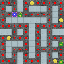
\includegraphics[scale=1.2]{abb/_envpics/example_red}
        \caption*{Rote Orbs}
        \label{fig:pic_chaser_redOrb}
    \end{minipage}
    %\caption{Chaser Environment - links unskaliert, rechts skaliert}
\end{figure}

\begin{figure}[htb!]
    \begin{minipage}{0.3\linewidth}
   \captionsetup{width=0.90\linewidth} 
        \centering
        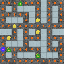
\includegraphics[scale=1.2]{abb/_envpics/example_orbSprite}
        \caption*{Default Spiel mit Orb-Sprite (Flammen)}
        \label{fig:pic_chaser_defaultOrbsprite}
    \end{minipage}
    \begin{minipage}{0.3\linewidth}
   \captionsetup{width=0.90\linewidth} 
        \centering
        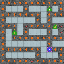
\includegraphics[scale=1.2]{abb/_envpics/example_changedSem_gelbOrb_Enemy}
        \caption*{Sprite-Tausch: großer Orb u. Geist}
        \label{fig:pic_chaser_semChange_yelOrb_enemy}
    \end{minipage}
    \begin{minipage}{0.3\linewidth}
   \captionsetup{width=0.90\linewidth} 
        \centering
        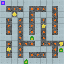
\includegraphics[scale=1.2]{abb/_envpics/example_changedSem_orb_wall}
        \caption*{Sprite-Tausch: kleiner Orb u. Wand}
        \label{fig:pic_chaser_semChange_Orb_wall}
    \end{minipage}
    %\caption{Chaser Environment - links unskaliert, rechts skaliert}
\end{figure}

\begin{figure}[htb!]
    \begin{minipage}{0.3\linewidth}
        \centering
        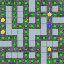
\includegraphics[scale=1.2]{abb/_envpics/example_green_250}
        \caption*{Orb-Farbe: grün:250}
        \label{fig:pic_chaser_green_250}
    \end{minipage}
    \begin{minipage}{0.3\linewidth}
        \centering
        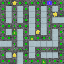
\includegraphics[scale=1.2]{abb/_envpics/example_green_200}
        \caption*{Orb-Farbe: grün:200}
        \label{fig:pic_chaser_green_200}
    \end{minipage}
    %\hfill
    \begin{minipage}{0.3\linewidth}
        \centering
        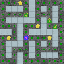
\includegraphics[scale=1.2]{abb/_envpics/example_green_150}
        \caption*{Orb-Farbe: grün:150}
        \label{fig:pic_chaser_green_150}
    \end{minipage}
    %\caption{Chaser Environment - links unskaliert, rechts skaliert}
\end{figure}

\newpage

\begin{figure}[htb!]
    \begin{minipage}{0.3\linewidth}
        \centering
        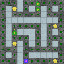
\includegraphics[scale=1.2]{abb/_envpics/example_green_100}
        \caption*{Orb-Farbe: grün:100}
        \label{fig:pic_chaser_green_100}
    \end{minipage}
    \begin{minipage}{0.3\linewidth}
        \centering
        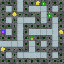
\includegraphics[scale=1.2]{abb/_envpics/example_green_50}
        \caption*{Orb-Farbe: grün:50}
        \label{fig:pic_chaser_green_50}
    \end{minipage}
    %\hfill
    \begin{minipage}{0.3\linewidth}
        \centering
        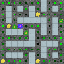
\includegraphics[scale=1.2]{abb/_envpics/example_green_rand}
        \caption*{Orb-Farbe: gruen, zufaellig 0-255}
        \label{fig:pic_chaser_green_random}
    \end{minipage}
    %\caption{Chaser Environment - links unskaliert, rechts skaliert}
\end{figure}

\begin{figure}[htb!]
   \captionsetup{width=0.3\linewidth} 
    \begin{minipage}{0.3\linewidth}
        \centering
        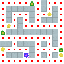
\includegraphics[scale=1.2]{abb/_envpics/example_whiteBG_red}
        \caption*{BG: weiß; \\ Orb: r:255, g:0, b:0}
        \label{fig:pic_chaser_whiteBG_red}
    \end{minipage}
    \begin{minipage}{0.3\linewidth}
        \centering
        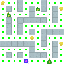
\includegraphics[scale=1.2]{abb/_envpics/example_whiteBG_green}
        \caption*{BG: weiß; \\ Orb: r:0, g:255, b:0}
        \label{fig:pic_chaser_whiteBG_green}
    \end{minipage}
    %\hfill
    \begin{minipage}{0.3\linewidth}
        \centering
        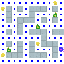
\includegraphics[scale=1.2]{abb/_envpics/example_whiteBG_blue}
        \caption*{BG: weiß; \\ Orb: r:0, g:0, b:255}
        \label{fig:pic_chaser_whiteBG_blue}
    \end{minipage}
    %\caption{Chaser Environment - links unskaliert, rechts skaliert}
\end{figure}


\paragraph{Beispiel Topologie eines dreischichtigen MLP}
\label{anh_mlp_L3}
Folgend ist ein Beispiel für den topologischen Aufbau eines Feed Forward MLP gegeben. 

\begin{figure}[htb!]
    \begin{minipage}{\linewidth}
        \centering
        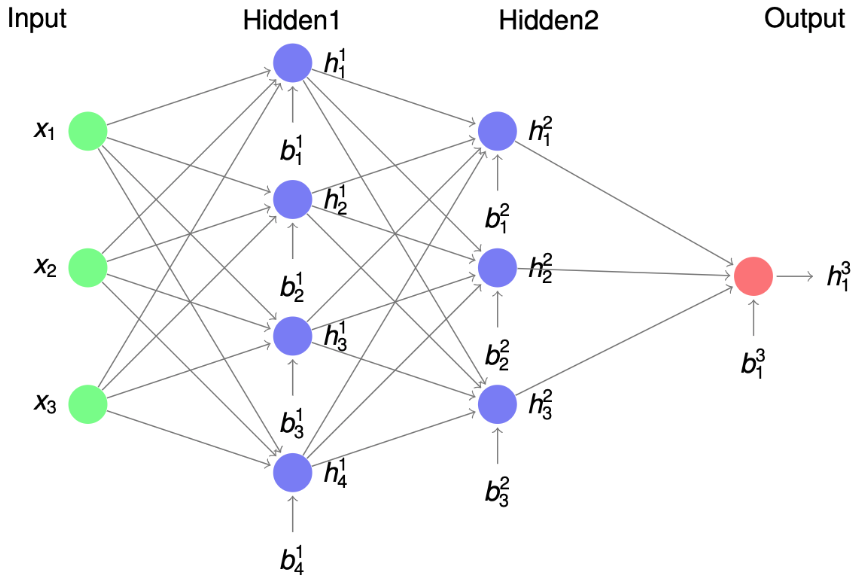
\includegraphics[scale=0.4]{abb/maucher_bsp_MLP}
        \caption*{Darstellung eines MLP mit drei Schichten \cite{maucher_ki_09}}
        \label{fig:pic_L3_mlp}
    \end{minipage}
\end{figure}
\newpage


\paragraph{Hyperparameter} \label{hyperparameter}
Folgend sind die verwendeten Hyperparameter in tabellarischer Form aufgearbeitet. 

\begin{center}
 \begin{table}[htb!]
 \begin{center}
  \begin{tabular}{c | c}
     Hyperparameter 		& Setting   \\ \hline \hline
     Learning Rate 		& 0,00025 \\ \hline 
     Entropie Koeffizient 	& 0,01 \\ \hline 
     Value Funciton Koeff.	& 0,5 \\ \hline 
     gamma $(\gamma)$	& 0,999 \\ \hline 
     lambda $(\lambda)$	& 0,95 \\ \hline 
     Anzahl Zeitschritte $T$	& 256  \\ \hline 
     Anzahl Minibatches	& 8  \\ \hline 
     Anzahl Epochen		& 3  \\ \hline 
     Clipping Range		& 0,2  \\ \hline 
  \end{tabular}
  \caption{Übersicht über die verwendeten Hyperparameter für PPO.}
  \label{tab:tab_durch_EXP_trainSetting3}
  \end{center}
 \end{table}
\end{center} 

\paragraph{Hardware} \label{hardware}
Folgend ist die verwendete Hardware in tabellarischer Form aufgelistet. Die Experimente werden auf dem Servern der Hochschule der Medien ausgeführt. Genauer wurde der GLaDOS-Server des Institute for Applied Artificial Intelligence verwendet. 

\begin{center}
 \begin{table}[htb!]
 \begin{center}
  \begin{tabular}{c | c}
    \hline
     	 				& GLaDOS   \\ \hline 
     Host 				& glados.mi.hdm-stuttgart.de        \\ \hline 
     CPU 				& i7-6950X (10-core) @ 3.0GHz \\ \hline 
     GPU				& 4x NVIDIA TITAN Xp 12GB        \\ \hline 
     Memory			& 128GB (8x 16GB) DDR4 PC2400 \\ \hline 
     
    \hline
  \end{tabular}
  \caption{Übersicht über die verwendete Hardware.}
  \label{tab:tab_durch_EXP_trainSetting3}
  \end{center}
 \end{table}
\end{center} 
\null\newpage

\paragraph{IMPALA-Architektur}\label{anh_impala_arch} \hfill \break
Folgend ist die IMPALA-Architektur aus dem Paper \cite{espeholt2018impala} dargestellt. Der Output dieser Architektur liefert den Input für sowohl die Policy-Approximation, als auch die Value-Function-Approximation.
\begin{figure}[htb!]
    \begin{minipage}{\linewidth}
        \centering
        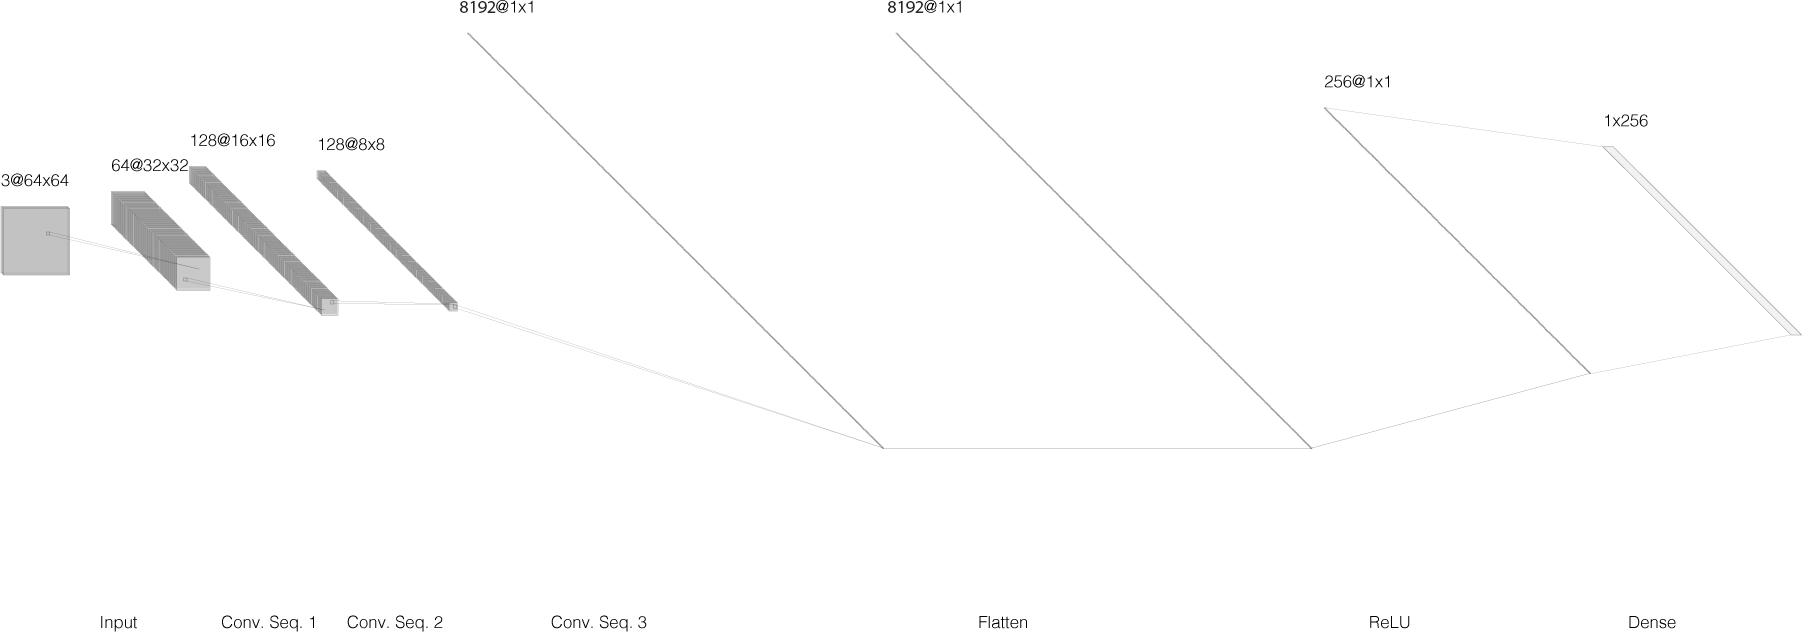
\includegraphics[angle=90,origin=c,scale=0.3]{abb/_networkArch/impala_net_arch}
        \caption*{Vereinfacht dargestellte IMPALA-Architektur}
        \label{fig:pic_impala_net_arch}
    \end{minipage}
\end{figure}
\vfill


\begin{figure}[htb!]
    \hspace*{-1.5cm}
    \begin{minipage}{\linewidth}
        \centering
        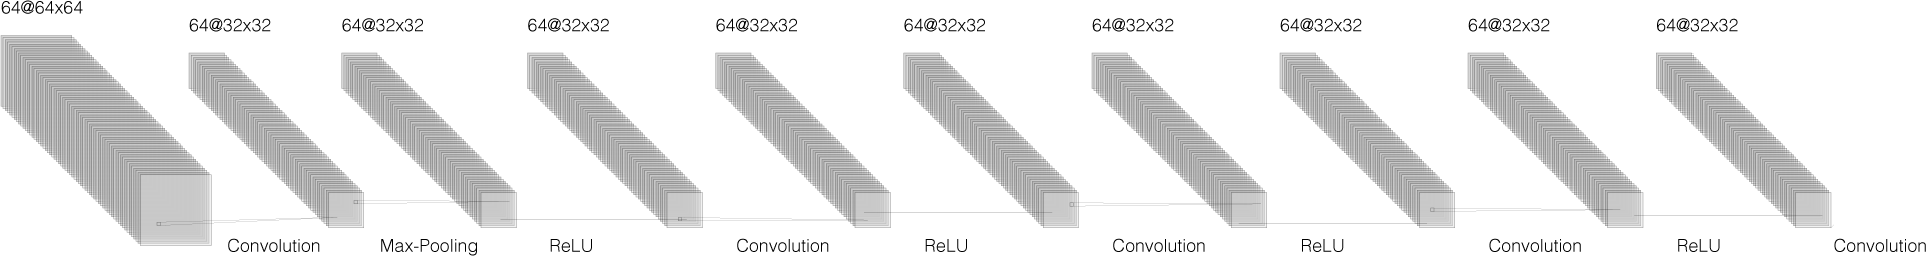
\includegraphics[scale=0.25]{abb/_networkArch/conv_seq_1}
        \caption*{Erste Convolutional Sequenz}
        \label{fig:pic_impala_net_arch}
    \end{minipage}
\end{figure}
\begin{figure}[htb!]
    \hspace*{-1.5cm}
    \begin{minipage}{\linewidth}
        \centering
        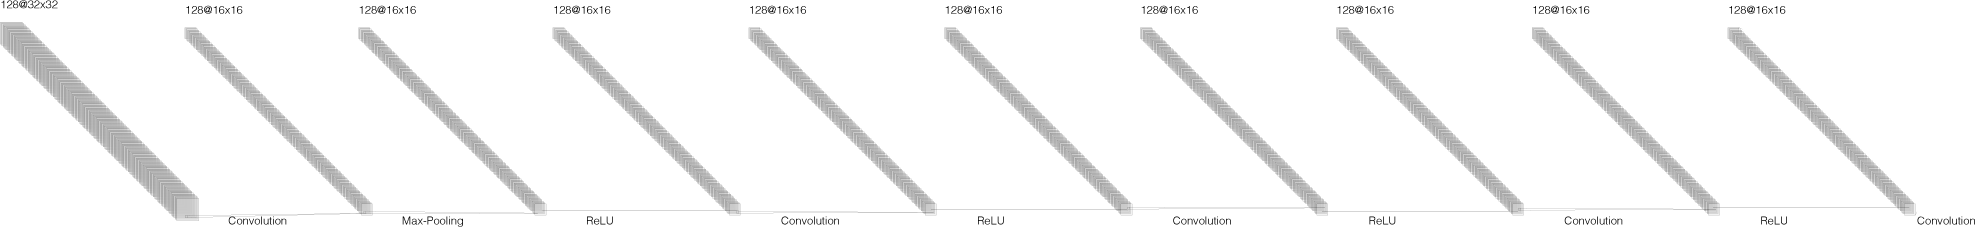
\includegraphics[scale=0.25]{abb/_networkArch/conv_seq_2}
        \caption*{Zweite Convolutional Sequenz}
        \label{fig:pic_impala_net_arch}
    \end{minipage}
\end{figure}
\begin{figure}[htb!]
    \hspace*{-1.5cm}
    \begin{minipage}{\linewidth}
        \centering
        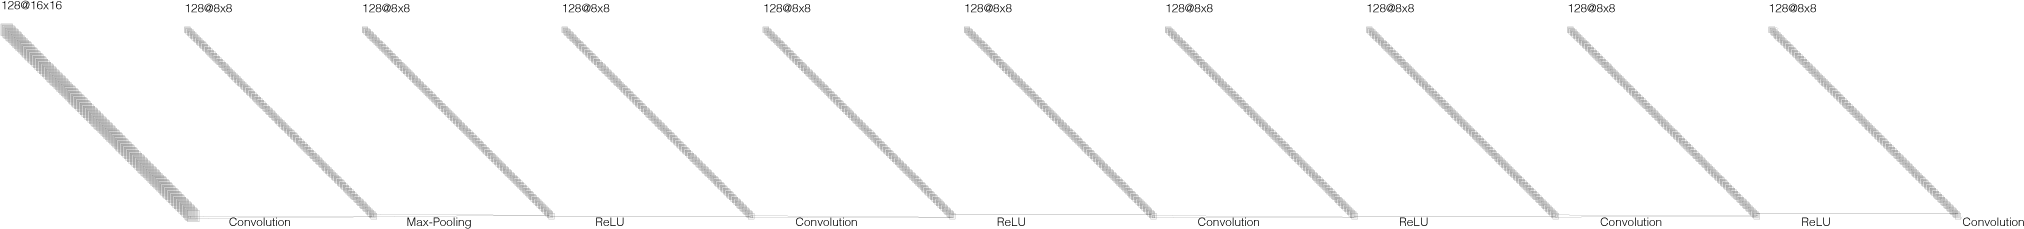
\includegraphics[scale=0.25]{abb/_networkArch/conv_seq_3}
        \caption*{Dritte Convolutional Sequenz}
        \label{fig:pic_impala_net_arch}
    \end{minipage}
\end{figure}

\paragraph{Experiment - 5 Mio. Zeitschritte, Grüner und Normaler Hintergrund}\label{anh_exp_5mio} \hfill \break
Folgend sind zwei Experimente mit zwei unterschiedlichen Agenten beschrieben. Hier werden beide Agenten für 5 Mio. Zeitschritte in einem einzigen Level trainiert. Das Training der beiden Agenten unterscheidet sich lediglich im verwendeten Hintergrund. Die genauen Trainingsbedingungen können Tabelle \ref{tab:tab_durch_EXP_trainSetting_anh_1} entnommen werden.

Abbildung \ref{fig:grph_green_80Mio_200lvl_15act_Training_evalAsTraining_5Mio1} zeigt das Training mit normalem Hintergrund. Abbildung \ref{fig:grph_green_80Mio_inflvl_15act_Training_evalAsTraining_5Mio2} zeigt das Training mit dem grünen Hintergrund.

\begin{figure}[htp!]
   \centering
   \captionsetup{width=0.45\linewidth} 
    \begin{minipage}{0.48\linewidth}
        \centering\
        \textbf{Normaler Hintergrund\\0 bis 15 Level}\par\medskip
        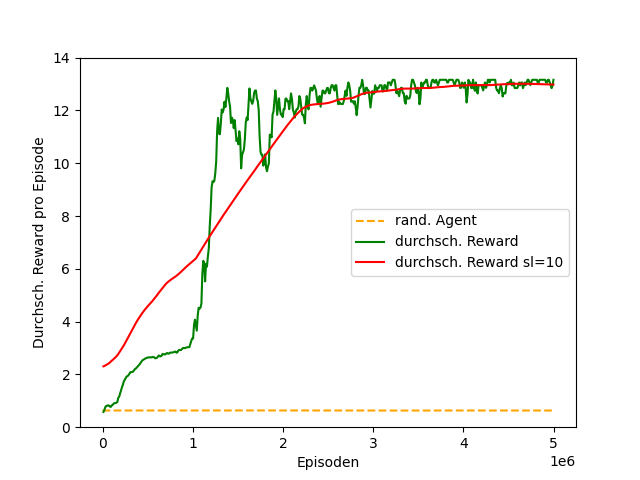
\includegraphics[scale=0.5]{abb/_graphen/tTimesteps_eprewmean_smooth_normal}
        \caption{Training mit normalem Hintergrund für 5 Mio. Zeitschritte.}
        \label{fig:grph_green_80Mio_200lvl_15act_Training_evalAsTraining_5Mio1} 
    \end{minipage}
    \centering
    \begin{minipage}{0.48\linewidth}
        \centering
        \textbf{Grüner Hintergrund\\0 bis 15 Level}\par\medskip
        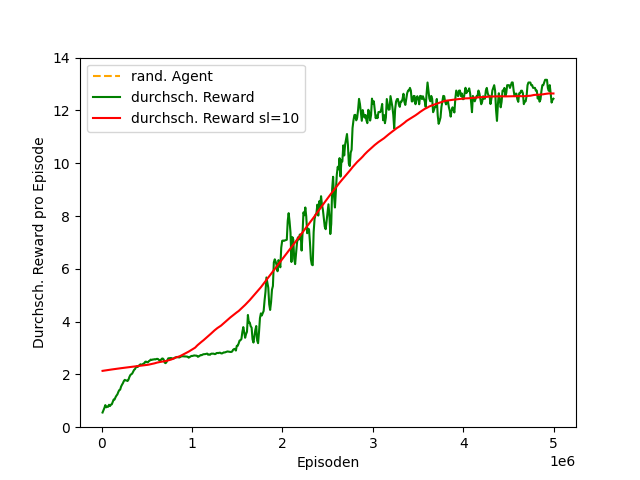
\includegraphics[scale=0.5]{abb/_graphen/tTimesteps_eprewmean_smooth_green} 
        \caption{Training mit grünem Hintergrund für 5 Mio. Zeitschritte.}
        \label{fig:grph_green_80Mio_inflvl_15act_Training_evalAsTraining_5Mio2}
    \end{minipage}
\end{figure}

\begin{center}
%\vskip-0.5cm
 \begin{table}[htb!]
 \begin{center}
  \begin{tabular}{ l c c c c }
    \hline
			       				& Zeitschritte 	& Anzahl Level 	& Hintergrund	 	& Farbe Orb \\ \hline \hline
     Training normaler Hintergrund  	& 5 Mio       	& 1		&  normal			& r:0, g:255, b:0 \\ \hline
     Training grüner Hintergrund   	& 5 Mio       	& 1 		&  r:0, g:255, g:0	& r:0, g:255, b:0 \\ \hline
    \hline
  \end{tabular}
  \caption{Übersicht über geltende Rahmenbedingungen in Training und Evaluation - 15.}
  \label{tab:tab_durch_EXP_trainSetting_anh_1}
  \end{center}
 \end{table}
\end{center} 
\vfill

\paragraph{Erfolgsrate Experiment zum Speichervermögen}\label{anh_exp_erfolgsrate}
Die folgende Tabelle zeigt die Erfolgsrate des jeweils letzten Checkpoints aller Agenten des Experiments \ref{par:durch_EXP_farbÄnd_Speichervermögen}.

\begin{center}
%\vskip-0.5cm
 \begin{table}[htb!]
 \begin{center}
  \begin{tabular}{ l c c  }
    \hline
	       				& Erfolgsrate \%, norm. BG 	& Erfolgsrate \%, grüner BG \\ \hline \hline
     Checkpoint 1  		&  98      			& 78		 \\ \hline
     Checkpoint 2  		& 90       			& 20		 \\ \hline
     Checkpoint 3  		& 76       			& 8		 \\ \hline
     Checkpoint 4  		& 56       			& 4		 \\ \hline
     Checkpoint 5  		& 54       			& 0		 \\ \hline
     Checkpoint 6 	 	& 64       			& 0		 \\ \hline
     Checkpoint 7  		& 52       			& 2		 \\ \hline
     Checkpoint 8	  	& 24       			& 0		 \\ \hline
     Checkpoint 9  		& 4       			& 4		 \\ \hline
     Checkpoint 10  		& 4       			& 4		 \\ \hline
     Checkpoint 11		& 34       			& 0		 \\ \hline
     Checkpoint 12		& 8       			& 0		 \\ \hline
     Checkpoint 13		& 4       			& 0		 \\ \hline
     Checkpoint 14  		& 10       			& 2		 \\ \hline
     Checkpoint 15  		& 8       			& 0		 \\ \hline
    \hline
  \end{tabular}
  \caption{Übersicht über die Erfolgsrate der Agenten mit normalem und grünem Hintergrund.}
  \label{tab:tab_durch_EXP_trainSetting5}
  \end{center}
 \end{table}
\end{center} 

\paragraph{Konzept des Convolutional Filtering}\label{anh_convConcept}
Die folgende Abbildung zeigt einen Schritt des Convolutional Filtering anhand eines zweidimensionalen Inputs. 
Diese Abbildung dient einer bildlichen Veranschaulichung des in Abschnitt \ref{absch_RL_convNets} vorgestellten Konzepts von Convolutional-Layers.

\begin{figure}[htb!]
 \centering
 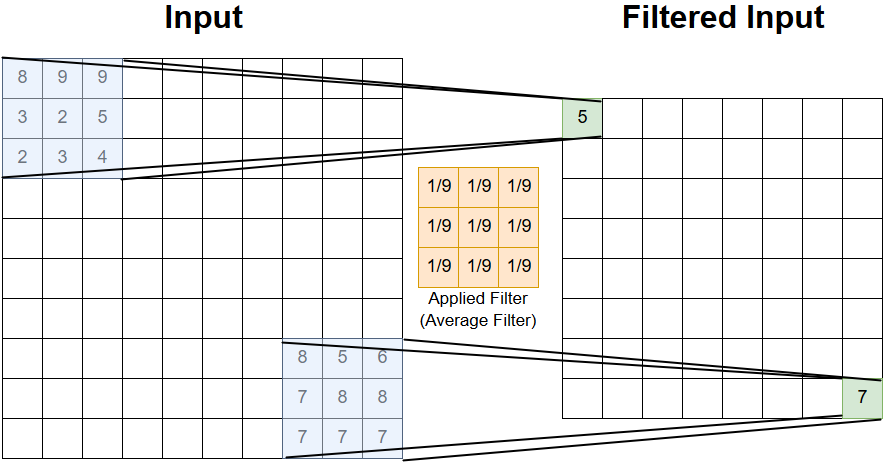
\includegraphics[scale=0.36]{abb/maucher_ConvolutionConcept}
 \caption[Beschreibung]{Darstellung des Konzepts des Convolutional Filtering \cite{maucher_nb_cnn}. }
\label{fig:maucher_cnn}
\end{figure}

\paragraph{Convolutional-Layer für 2D-Input}\label{anh_conv2d}
Die folgende Abbildung zeigt eine Berechnung eines Features aus einem zweidimensionalen Convolutional-Layer. Weiter zeigt das Bild die jeweiligen geteilten Gewichte (hier in rot und blau). Die Kernel Size ist hier $[3 \times 3]$. Somit teilen sich die Neuronen $x_{11}, x_{12}, ..., x_{33}$ eine Gewichtsmatrix. Dasselbe gilt für jeden Block des Inputs der Größe $[3 \times 3]$, wie in Abbildung \ref{fig:maucher_cnn2d} ersichtlich. 

\begin{figure}[htb!]
 \centering
 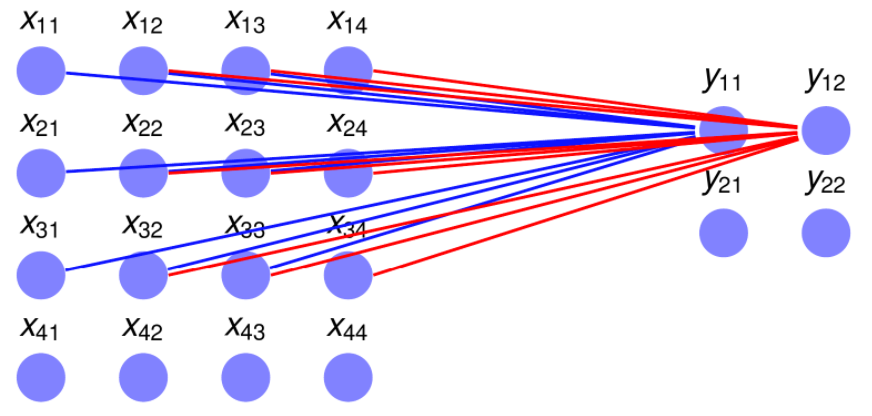
\includegraphics[scale=0.4]{abb/maucher_2dConvLayer}
 \caption[Beschreibung]{Darstellung einer Single Feature Map, extrahiert aus einem einkanäligen, zweidimensionalen Convolutional-Layer \cite{maucher_nb_cnn}. }
\label{fig:maucher_cnn2d}
\end{figure}


